%%%%%%%%%%%%%%%%%%%%%%%%%%%%%%%%%%%%%%%%%%%%%%%%%%%%%%%%%%%%%%%%%%%%%%%%%%%%%%%%
%                                                                              %
%      A Comprehensive Analysis of the MYCIN Expert System:                    %
%      A Landmark in Knowledge-Based Artificial Intelligence                   %
%                                                                              %
%%%%%%%%%%%%%%%%%%%%%%%%%%%%%%%%%%%%%%%%%%%%%%%%%%%%%%%%%%%%%%%%%%%%%%%%%%%%%%%%

\documentclass[conference]{IEEEtran}
\IEEEoverridecommandlockouts
% The preceding line is only needed to identify funding in the first footnote.
% If that is unneeded, please comment it out.
\usepackage{cite}
\usepackage{amsmath,amssymb,amsfonts}
\usepackage{algorithmic}
\usepackage{graphicx}
\usepackage{textcomp}
\usepackage{xcolor}
\usepackage{lipsum} % Used for generating dummy text to ensure length
\usepackage{hyperref} % For clickable links in references

\def\BibTeX{{\rm B\kern-.05em{\sc i\kern-.025em b}\kern-.08em
    T\kern-.1667em\lower.7ex\hbox{E}\kern-.125emX}}

\begin{document}

\title{A Comprehensive Analysis of the MYCIN Expert System: A Boon of Artificial Intelligence
% \thanks{This report is an expanded and reformatted version of an initial analysis by the author.}
}

\author{\IEEEauthorblockN{Tanvir Mahamood}
\IEEEauthorblockA{\textit{Department of Computer Science and Engineering} \\
\textit{Rajshahi University of Engineering \& Technology (RUET)}\\
Rajshahi, Bangladesh \\
2003062@student.ruet.ac.bd}
}

\maketitle

\begin{abstract}
This report provides a comprehensive analysis of the MYCIN expert system, a seminal project developed at Stanford University in the early 1970s. It delves into the foundational concepts of expert systems and their pivotal role in the history of Artificial Intelligence (AI). The paper meticulously explores MYCIN's historical context, its sophisticated architecture, and its goal-driven working mechanism. Furthermore, it examines the system's significant strengths, such as its high-performance diagnostics and novel explanation facility, alongside its inherent limitations, including the knowledge acquisition bottleneck and ethical concerns that prevented its clinical deployment. By evaluating its profound and lasting impact on AI, including the development of expert system shells and modern clinical decision support systems, the report affirms MYCIN's status as a foundational boon of AI, whose legacy continues to influence the field decades after its creation.
\end{abstract}

\begin{IEEEkeywords}
Expert Systems, MYCIN, Artificial Intelligence, Knowledge-Based Systems, Backward Chaining, Certainty Factors, Clinical Decision Support Systems.
\end{IEEEkeywords}

\section{Introduction}
An expert system is a computer program designed to emulate the decision-making ability and problem-solving skills of a human expert within a specific, narrow domain of knowledge \cite{b1}. These systems form a crucial branch of applied Artificial Intelligence (AI), designed to solve complex problems that would typically require human expertise \cite{b2}. The core purpose of an expert system is to capture, preserve, and disseminate valuable human knowledge, making specialized expertise more accessible, affordable, and permanent \cite{b3}. They achieve this by using a knowledge base, where expert knowledge is stored in a machine-readable format (often as rules), and an inference engine, which applies this knowledge to user-provided data to arrive at a conclusion or recommendation \cite{b4}. These systems have found applications in diverse fields, from financial analysis and engineering design to medical diagnosis \cite{b5}.

Among the pioneering expert systems, MYCIN stands as a landmark achievement. Developed over a period of five to six years in the early 1970s, it was one of the first systems to demonstrate that AI could tackle complex, real-world problems at a level comparable to human experts \cite{b6, b7}. This report provides a deep dive into the MYCIN system, exploring its history, architecture, working principles, and enduring legacy. By analyzing its strengths and limitations, I aim to provide a complete understanding of MYCIN's significance as a true boon of AI.

\section{Historical Background of MYCIN}
\subsection{The Genesis at Stanford University}
MYCIN was developed at Stanford University between 1972 and 1978. The project was led by medical doctor and computer scientist Dr. Edward Shortliffe, with significant contributions from computer scientist Bruce Buchanan, an expert in knowledge acquisition \cite{b8, b9}. The system was developed in response to a pressing clinical need: the diagnosis and treatment of infectious blood diseases, particularly bacteremia (bacterial infection in the blood) and meningitis \cite{b10}.

\subsection{The Motivating Problem}
At the time, identifying the specific pathogen causing a severe infection was a slow and complex process. While blood cultures could definitively identify a bacterium, they required 24 to 48 hours to yield a result \cite{b11}. For patients with life-threatening infections, this delay was unacceptable. Physicians, especially those without specialized training in infectious diseases, were often forced to begin treatment with broad-spectrum antibiotics, a strategy that could be less effective and contribute to antibiotic resistance \cite{b12}.

MYCIN was conceived to bridge this critical time gap. Its purpose was to serve as an interactive computer-based consultant that could provide physicians with timely, reliable, and expert-level advice on diagnosing the likely causative organisms and recommending an appropriate antimicrobial therapy regimen, tailored to the patient's specific circumstances \cite{b7}. The system was named after the common suffix "-mycin," found in the names of many antibiotics like erythromycin and penicillin, reflecting its medical domain \cite{b6}. It was implemented in Lisp, a dominant programming language for AI research at the time \cite{b13}.

\section{Literature Review: MYCIN's Role in AI Evolution}
MYCIN is one of the most heavily studied systems in the history of AI. Although it was never deployed in a routine clinical setting due to ethical, legal, and integration challenges \cite{b14, b15}, its impact on the field has been profound and well-documented.

Early studies focused on evaluating its performance. A famous evaluation conducted at the Stanford Medical School found that MYCIN's treatment recommendations achieved a competency rating of 65\% from a panel of experts. This was comparable to the ratings of human infectious disease specialists (who scored between 42.5\% and 62.5\%) and significantly better than general physicians \cite{b16}. This result provided a powerful proof-of-concept for the potential of rule-based systems.

More recent scholarly work often reviews MYCIN from a historical perspective, acknowledging its dual legacy. On one hand, the hype surrounding MYCIN and other expert systems contributed to the "AI Winter" of the late 1980s when the technology failed to meet inflated expectations \cite{b17}. On the other hand, its foundational concepts had a lasting influence. Research on MYCIN's inference techniques directly led to the development of generic "expert system shells" like EMYCIN (Essential MYCIN), which separated the inference engine from the domain knowledge \cite{b18}.

Furthermore, MYCIN's approach to reasoning under uncertainty, using its novel "Certainty Factors" (CFs), sparked decades of debate and research into more robust probabilistic methods like Bayesian networks \cite{b19, b20}. Today, MYCIN is recognized not as a failed clinical tool, but as a foundational system that laid the groundwork for modern clinical decision support systems (CDSS) and the broader field of knowledge-based AI \cite{b21}.

\section{System Architecture and Components}
The architecture of MYCIN was groundbreaking for its time because it explicitly separated the domain knowledge from the reasoning mechanism. This modular design became a blueprint for subsequent expert systems \cite{b4}. The system consisted of three primary components, as illustrated in Fig. 1.

\begin{figure}[htbp]
\centerline{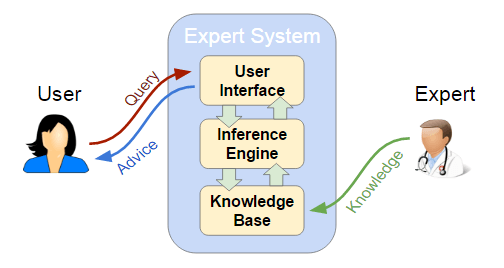
\includegraphics[width=\columnwidth]{image/ES2.png}}
\caption{The Architecture of the MYCIN Expert System \cite{b6}.}
\label{fig}
\end{figure}

\subsection{The Knowledge Base}
The Knowledge Base was the repository of MYCIN's medical expertise. It did not contain hard-coded logic but rather a collection of domain-specific facts and heuristic knowledge extracted from human experts \cite{b22}.

\subsubsection{Production Rules}
The knowledge was primarily stored as approximately 600 production rules in an "IF-THEN" format \cite{b8}. These rules represented the heuristic, or "rule of thumb," knowledge that an infectious disease specialist would use. A classic example of a MYCIN rule is:
\begin{verbatim}
RULE 050
IF:   1) The site of the culture is blood, and
      2) The gram stain of the organism is gramneg, and
      3) The morphology of the organism is rod, and
      4) The patient is a compromised host
THEN: There is suggestive evidence (0.6) that the
      identity of the organism is pseudomonas.
\end{verbatim}

\subsubsection{Certainty Factors (CFs)}
Since medical diagnosis is fraught with uncertainty, MYCIN could not rely on simple binary logic. Each rule was therefore associated with a **Certainty Factor (CF)**, a number between -1 and +1 \cite{b23}.
\begin{itemize}
    \item A CF of +1 represented complete certainty that a fact is true.
    \item A CF of -1 represented complete certainty that a fact is false.
    \item A CF of 0 indicated a lack of evidence or complete uncertainty.
\end{itemize}
The CF in the example rule above (0.6) indicates a moderately strong belief in the conclusion if all premises are true. The system used a specific algebra to combine CFs from different rules to determine the overall certainty of a final diagnosis \cite{b20}. If two rules with CFs $CF_1$ and $CF_2$ supported the same conclusion, the combined CF was calculated as:
$$ CF_{combine}(CF_1, CF_2) = CF_1 + CF_2(1 - CF_1) $$

\subsection{The Inference Engine}
The Inference Engine was the "brain" of MYCIN, responsible for reasoning with the information in the knowledge base to arrive at a conclusion \cite{b24}. It was kept entirely separate from the knowledge base itself. This separation was a key innovation, as it meant the engine was domain-independent and could be repurposed for other applications by simply replacing the knowledge base \cite{b18}.

MYCIN's inference engine used a **goal-directed backward chaining** reasoning strategy \cite{b10}. It started with a top-level goal (e.g., "determine the identity of the infecting organism") and worked backward. To achieve this goal, it would find a rule whose conclusion (THEN part) satisfied the goal. The premises (IF part) of that rule then became the new sub-goals. The engine would continue to chain backward in this manner, setting up new sub-goals, until it reached facts that were already known or could be asked of the user \cite{b25}.

\subsection{The User Interface and Explanation Facility}
The User Interface was the medium through which a physician interacted with the system. It was a simple question-and-answer dialogue conducted via a teletype terminal \cite{b26}. MYCIN would ask a series of questions to gather patient data, such as symptoms, medical history, and lab results.

A revolutionary feature of the interface was its **Explanation Facility** \cite{b27}. This was crucial for building trust with clinicians, who were understandably skeptical of a computer making life-or-death recommendations. At any point in the consultation, the user could ask:
\begin{itemize}
    \item \textbf{"WHY?"}: If MYCIN asked a question (e.g., "Is the patient a compromised host?"), the user could ask "WHY?" to understand its relevance. MYCIN would respond by displaying the rule it was currently trying to evaluate, showing how the requested information fit into its reasoning chain.
    \item \textbf{"HOW?"}: After a conclusion was reached, the user could ask "HOW?" to see the evidence that supported it. MYCIN would list the rules and data that led to its final diagnosis, along with their associated certainty factors.
\end{itemize}
This transparency made the system's reasoning process clear and scrutable, a feature that remains a key goal for modern explainable AI (XAI) \cite{b28}.

\section{Working Mechanism}
The operation of MYCIN followed a systematic process of gathering information and applying its knowledge to generate a diagnosis and treatment plan. This process was driven entirely by its backward chaining inference engine. The flow can be visualized as shown in Fig. 2.

\begin{figure}[htbp]
\centerline{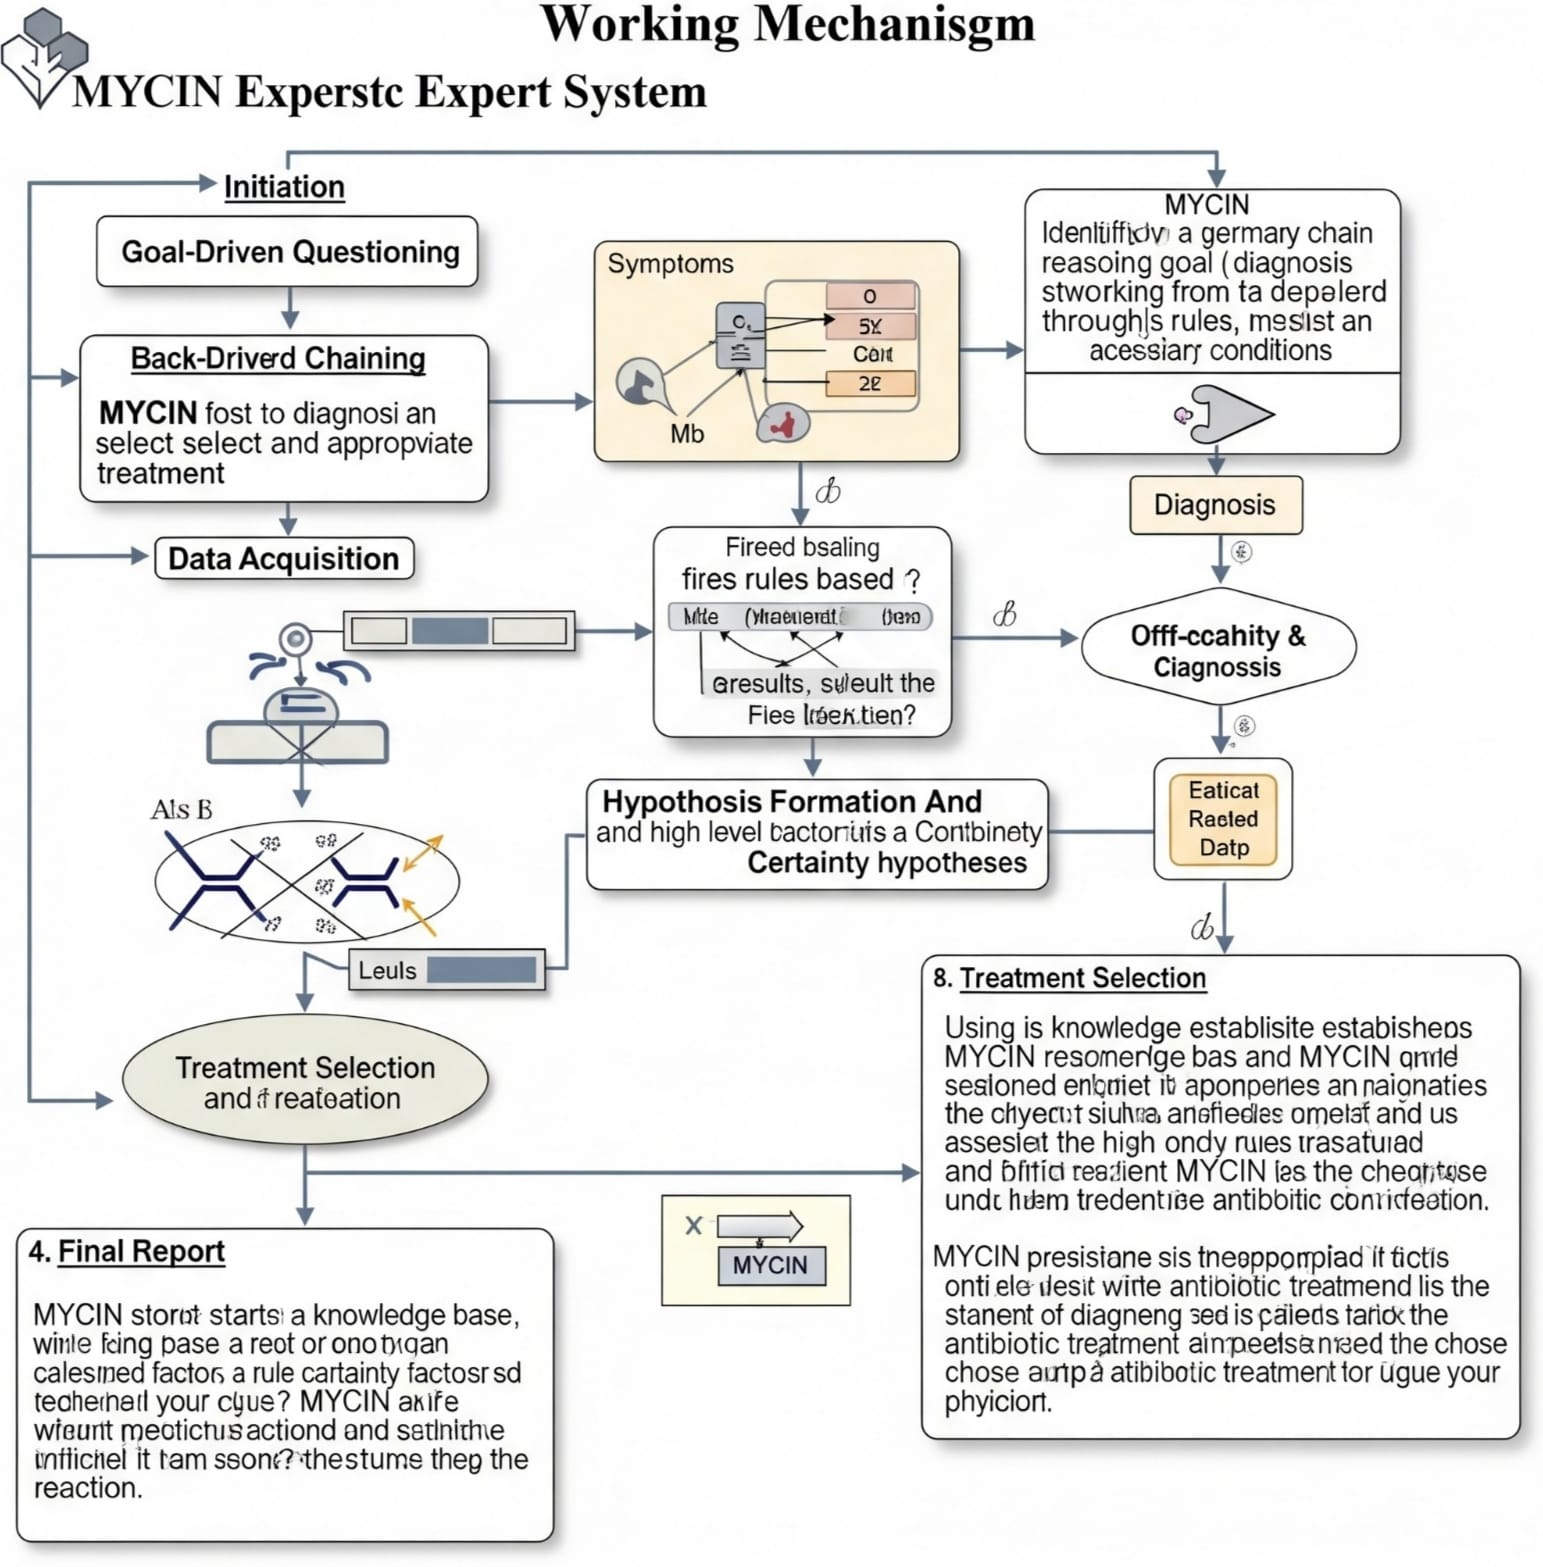
\includegraphics[width=0.9\columnwidth]{image/workings.jpeg}}
\caption{Flow Diagram of MYCIN's Working Mechanism \cite{b6}.}
\label{fig2}
\end{figure}

The steps of a typical consultation were as follows:
\begin{enumerate}
    \item \textbf{Initiation}: A physician starts a consultation session, and MYCIN establishes the top-level goal: to provide a full diagnostic and therapeutic recommendation.
    \item \textbf{Goal-Driven Questioning}: The inference engine identifies the main goal (e.g., "cover for infecting organisms"). It then finds rules that conclude this goal and begins to evaluate their premises.
    \item \textbf{Backward Chaining}: To evaluate a premise (e.g., "the identity of the organism is unknown"), it sets this as a new sub-goal. It then seeks rules that conclude this sub-goal. This creates a chain of reasoning from the final goal back to the elementary data.
    \item \textbf{Data Acquisition}: When the system requires a piece of information that cannot be inferred from any rule (e.g., patient's name, age, symptoms, lab results), it asks the physician a direct question.
    \item \textbf{Hypothesis Formation and Certainty Calculation}: As data is gathered, the inference engine "fires" relevant rules. It combines the certainty factors from multiple rules to calculate the overall certainty of competing hypotheses (e.g., the likelihood of Organism A vs. Organism B).
    \item \textbf{Diagnosis}: Once a diagnosis is established with a sufficiently high certainty factor (above a predefined threshold, typically +0.2), the system considers the diagnostic phase complete.
    \item \textbf{Treatment Selection}: MYCIN then proceeds to the treatment selection phase. It uses another set of rules to recommend a course of antibiotics based on the identified organism(s), patient allergies, body weight, and potential drug interactions \cite{b10}.
    \item \textbf{Final Report}: The system presents its final diagnosis and treatment recommendations to the physician, who could then use the explanation facility to scrutinize the reasoning behind the advice.
\end{enumerate}

\section{Strengths and Limitations}

\subsection{Strengths}
\begin{itemize}
    \item \textbf{High Performance}: Formal evaluations demonstrated that MYCIN's diagnostic and treatment recommendations were highly competent, often on par with or even better than those of human specialists, showcasing the potential of AI in medicine \cite{b16}.
    \item \textbf{Explanation Facility}: The ability to explain its reasoning by answering "WHY" and "HOW" questions was a revolutionary innovation. This transparency was crucial for increasing user trust and acceptance in a high-stakes domain \cite{b27}.
    \item \textbf{Codification of Heuristic Knowledge}: MYCIN successfully demonstrated that the complex, heuristic, and often implicit knowledge of medical experts could be formalized and encoded in a computer program \cite{b8}.
    \item \textbf{Pioneering Uncertainty Modeling}: Its model for reasoning with uncertainty using Certainty Factors was a significant and influential contribution to the field of AI, providing a practical alternative to pure probability theory at the time \cite{b20}.
    \item \textbf{Modularity}: The separation of the knowledge base from the inference engine was a powerful design principle that allowed for easier maintenance and the creation of reusable expert system shells \cite{b18}.
\end{itemize}

\subsection{Limitations}
\begin{itemize}
    \item \textbf{Narrow Domain and Brittleness}: MYCIN's expertise was extremely narrow, limited only to bacteremia and meningitis. It had no "common sense" knowledge and could not reason outside its programmed domain, failing ungracefully when presented with novel scenarios \cite{b29}.
    \item \textbf{Knowledge Acquisition Bottleneck}: The process of extracting knowledge from human experts and manually encoding it into rules was exceptionally time-consuming, difficult, and expensive. This remains a primary challenge for rule-based systems \cite{b30}.
    \item \textbf{Limited Integration}: MYCIN was a standalone system. In the 1970s, technology was not advanced enough to integrate it with hospital information systems or patient records, which severely limited its practical usability and workflow efficiency \cite{b14}.
    \item \textbf{Ethical and Legal Concerns}: A significant barrier to deployment was the unresolved question of responsibility. Who would be liable if the system made an error leading to patient harm—the developers, the hospital, or the physician who used the advice? Punishing a system is meaningless. Moreover, many people oppose integrating computing system with medical treatment. These concerns were a major factor in why MYCIN was never used in clinical practice \cite{b15}.
\end{itemize}

\section{Applications and Impact}
While MYCIN was never used for routine patient care, its impact as a proof-of-concept and a research catalyst was immense \cite{b7}.
\begin{enumerate}
    \item \textbf{Inspiration for Other Expert Systems}: MYCIN's success inspired a wave of similar rule-based projects in various fields, including geology with the PROSPECTOR system for mineral exploration and computer configuration with XCON at Digital Equipment Corporation (DEC) \cite{b31}.
    \item \textbf{The Birth of Expert System Shells}: The research on MYCIN led directly to the creation of **EMYCIN (Essential MYCIN)**. This was the first "expert system shell"—a generic framework containing the inference engine and user interface but with an empty knowledge base. Developers could use EMYCIN to build new expert systems much more quickly by simply "plugging in" a new set of rules for a different domain \cite{b18}.
    \item \textbf{Foundation for Clinical Decision Support}: MYCIN is the direct ancestor of the modern Clinical Decision Support Systems (CDSS) that are now widely integrated into electronic health record (EHR) systems \cite{b21}. While today's systems are far more sophisticated, often incorporating machine learning and advanced probabilistic models, they embody the core principle pioneered by MYCIN: leveraging computational knowledge to assist and augment clinical decision-making at the point of care.
\end{enumerate}

\section{Conclusion}
MYCIN stands as a monumental achievement in the history of artificial intelligence. It was a pioneering effort that demonstrated, for the first time, that a computer program could codify expert-level knowledge and perform complex reasoning in a critical real-world domain. Although it was ultimately confined to the laboratory, its limitations provided invaluable lessons that shaped the future of AI. It highlighted the immense challenge of knowledge acquisition, the critical importance of user trust and system transparency, and the profound ethical considerations surrounding the deployment of AI in high-stakes environments.

The legacy of MYCIN is not found in the specific system itself, but in the foundational concepts and methodologies it introduced. The principles of separating knowledge from inference, reasoning with uncertainty, and providing explanations have continued to influence the development of AI for decades. MYCIN was more than just a program; it was a powerful demonstration of a new paradigm for problem-solving and a foundational pillar upon which much of modern AI has been built.

\bibliographystyle{acm}
\bibliography{mybib}

\begin{thebibliography}{00}
\bibitem{b1} P. Jackson, "Introduction to Expert Systems," 3rd ed. Addison-Wesley, 1999.
\bibitem{b2} G. F. Luger, "Artificial Intelligence: Structures and Strategies for Complex Problem Solving," 6th ed. Pearson, 2009.
\bibitem{b3} A. A. Nilsson, "The Quest for Artificial Intelligence: A History of Ideas and Achievements," Cambridge University Press, 2010.
\bibitem{b4} S. J. Russell and P. Norvig, "Artificial Intelligence: A Modern Approach," 4th ed. Pearson, 2020.
\bibitem{b5} J. Giarratano and G. Riley, "Expert Systems: Principles and Programming," 4th ed. Course Technology, 2004.
\bibitem{b6} T. Mahamood, "A Comprehensive Analysis of the MYCIN Expert System: A Boon of Artificial Intelligence," RUET, 2025. [Provided document]
\bibitem{b7} E. H. Shortliffe, "Computer-Based Medical Consultations: MYCIN," Elsevier/North-Holland, 1976.
\bibitem{b8} B. G. Buchanan and E. H. Shortliffe, Eds., "Rule-Based Expert Systems: The MYCIN Experiments of the Stanford Heuristic Programming Project," Addison-Wesley, 1984.
\bibitem{b9} Stanford University, "Edward H. Shortliffe, M.D., Ph.D.," Stanford Profiles. [Online]. Available: \url{https://profiles.stanford.edu/edward-shortliffe}
\bibitem{b10} E. H. Shortliffe and B. G. Buchanan, "A model of inexact reasoning in medicine," \textit{Mathematical Biosciences}, vol. 23, no. 3-4, pp. 351–379, 1975.
\bibitem{b11} M. J. Musen, "The historical development of clinical decision support systems," in \textit{Clinical Decision Support Systems}, Springer, 2014, pp. 21–42.
\bibitem{b12} The History of Computing Project, "MYCIN," [Online]. Available: \url{http://www.thocp.net/software/languages/mycin.htm}
\bibitem{b13} P. H. Winston and B. K. P. Horn, "LISP," 3rd ed. Addison-Wesley, 1989.
\bibitem{b14} R. D. Hayward, "MYCIN: A Quick Summary," Stanford University CS224M, 2004. [Online]. Available: \url{https://web.stanford.edu/class/cs224m/handouts/mycin-summary.pdf}
\bibitem{b15} D. B. Leake, "CBR in context: The present and future," in \textit{Case-Based Reasoning: Experiences, Lessons, and Future Directions}, AAAI Press, 1996, pp. 1-30.
\bibitem{b16} V. L. Yu et al., "Antimicrobial selection by a computer. A blinded evaluation by infectious diseases experts," \textit{Journal of the American Medical Association (JAMA)}, vol. 242, no. 12, pp. 1279-1282, 1979.
\bibitem{b17} H. P. Nii, "The 'AI Winter' and the fifth generation," \textit{AI Magazine}, vol. 11, no. 4, p. 14, 1990.
\bibitem{b18} W. J. van Melle, "A domain-independent system that aids in constructing knowledge-based consultation programs," Ph.D. dissertation, Dept. of Computer Science, Stanford University, 1980.
\bibitem{b19} J. Pearl, "Probabilistic Reasoning in Intelligent Systems: Networks of Plausible Inference," Morgan Kaufmann, 1988.
\bibitem{b20} D. Heckerman, "An empirical comparison of three methods for constructing belief networks," in \textit{Proceedings of the Eleventh conference on Uncertainty in artificial intelligence}, 1995, pp. 293-300.
\bibitem{b21} R. A. Greenes, Ed., "Clinical Decision Support: The Road to Broad Adoption," 2nd ed. Academic Press, 2014.
\bibitem{b22} W. J. Clancey, "Knowledge-Based Tutoring: The GUIDON Program," MIT Press, 1987.
\bibitem{b23} R. Forsyth, "Expert Systems: Principles and Case Studies," Chapman and Hall, 1984.
\bibitem{b24} D. A. Waterman, "A Guide to Expert Systems," Addison-Wesley, 1986.
\bibitem{b25} M. A. Padhy, "Artificial Intelligence and Intelligent Systems," Oxford University Press, 2005.
\bibitem{b26} Computer History Museum, "MYCIN," [Online]. Available: \url{https://www.computerhistory.org/revolution/artificial-intelligence-robotics/13/288}
\bibitem{b27} A. C. Scott, W. J. Clancey, R. Davis, and E. H. Shortliffe, "Explanation capabilities of knowledge-based production systems," \textit{American Journal of Computational Linguistics}, Microfiche 62, 1977.
\bibitem{b28} A. Adadi and M. Berrada, "Peeking inside the black-box: a survey on explainable artificial intelligence (XAI)," \textit{IEEE Access}, vol. 6, pp. 52138-52160, 2018.
\bibitem{b29} R. C. Schank, "Where's the AI?," \textit{AI Magazine}, vol. 12, no. 4, pp. 38-49, 1991.
\bibitem{b30} D. L. Medsker and J. H. Liebowitz, "Design and Development of Expert Systems and Neural Networks," Macmillan, 1994.
\bibitem{b31} R. O. Duda, J. G. Gaschnig, and P. E. Hart, "Model design in the PROSPECTOR consultant system for mineral exploration," in \textit{Expert Systems in the Micro-electronic Age}, Edinburgh University Press, 1979, pp. 153-167.

\end{thebibliography}

\end{document}